\section{PINN Implementation of Traveltime Inversion}
\label{sec:pinn_implementation}

I perform PINN tomography using 14,400 picked traveltimes (\figref{fig:data}). The traveltime network has 5 hidden layers with 50 neurons each as opposed to the velocity network which has 4 hidden layers of 20 neurons. I constrain the velocity predictions with an upper bound of 2.2 km/s based on the findings from the experiments conducted on the region previously. As in the synthetic examples, I give the data fitting term 100 times more weight than the eikonal loss. Because of the data shows a high signal- to-noise ratio (\figref{fig:shot_gather_fa}), this strategy ensures robust convergence. I use 50,000 Adam with a minibatch size of 100, plus less than 35,000 L-BFGS iterations to train the PINN (\figref{fig:adam_LBFGS}).

\begin{figure}
 \centering
 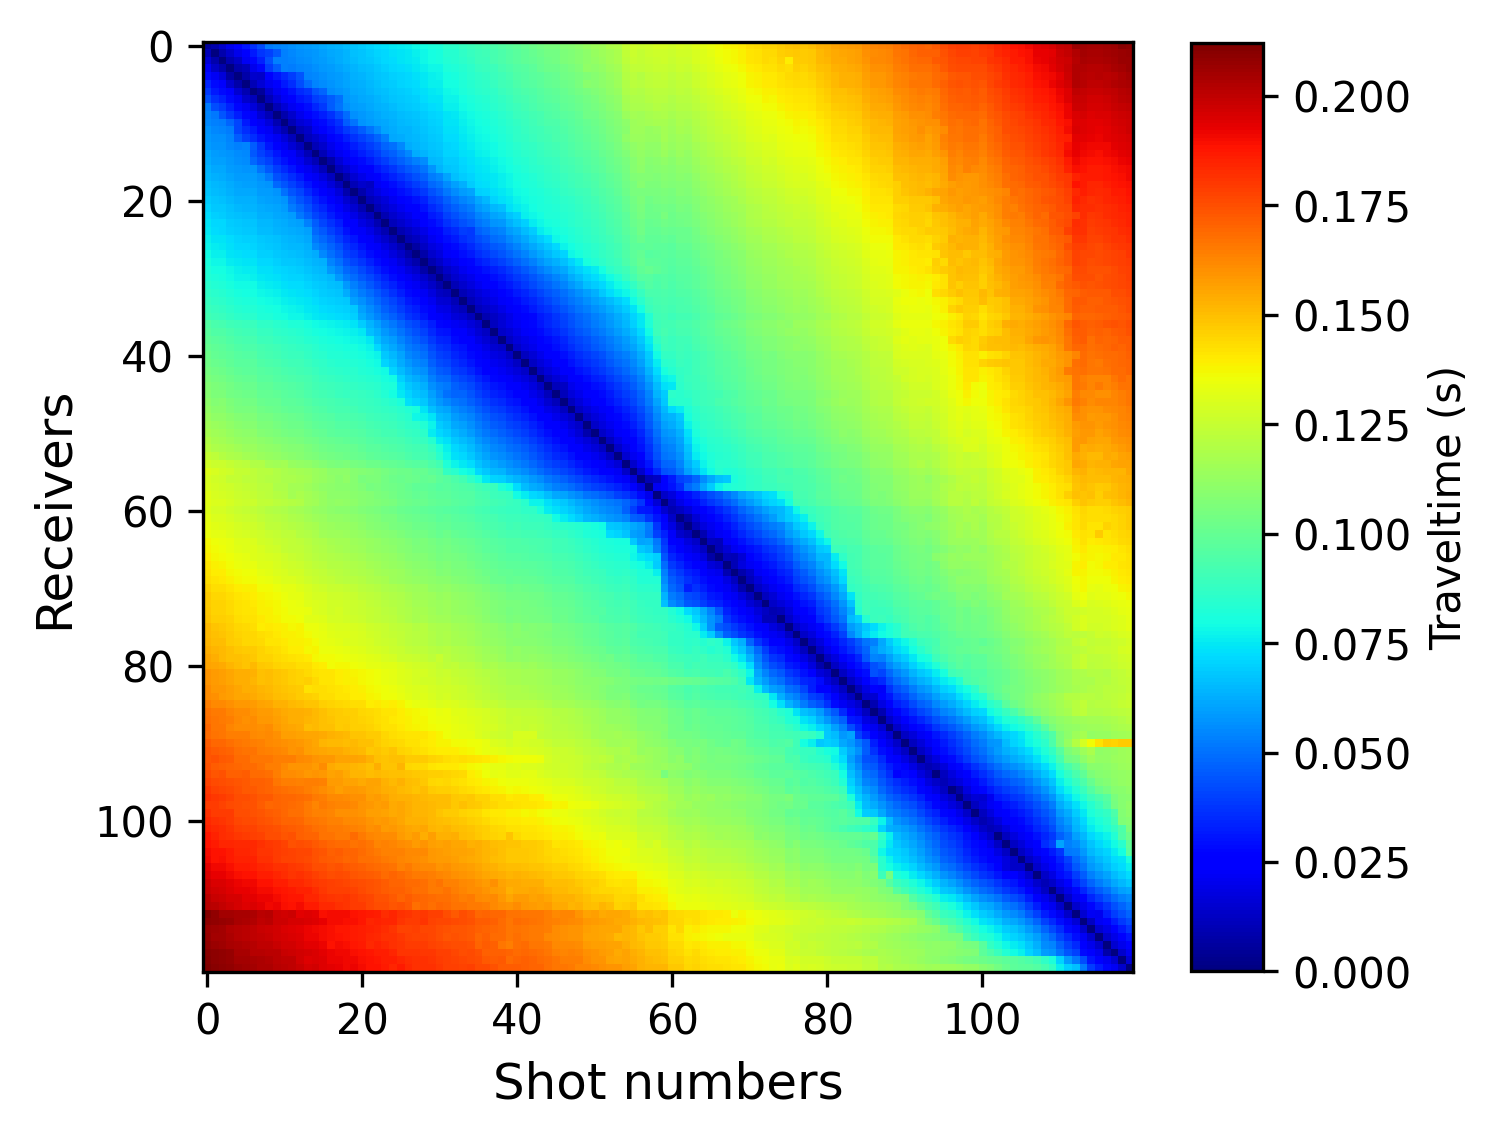
\includegraphics[width=0.9\textwidth]{figures/chap04_field_data/data} 
 \caption{Image representation of the field data. There are 120 shots each having 120 observed traveltimes that are placed in rows to form the image.}
 \label{fig:data}
\end{figure}

 \begin{figure}
       \centering
       \begin{subfigure}[b]{.45\textwidth}
               \centering
               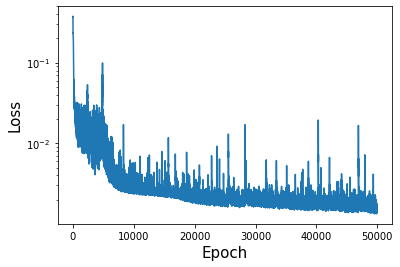
\includegraphics[width=0.9\textwidth, height=0.7\textwidth]{figures/chap04_field_data/field_data_Adam.png} 
               \caption{}
               \label{fig:adam}
       \end{subfigure}%
       ~
       \begin{subfigure}[b]{.45\textwidth}
               \centering
               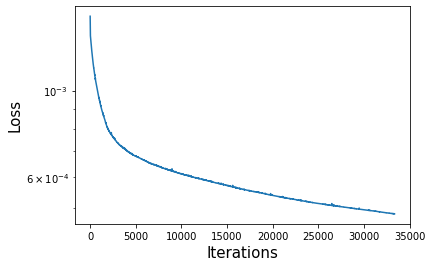
\includegraphics[width=0.9\textwidth,
               height=0.7\textwidth]{figures/chap04_field_data/field_data_LBFGS}
               \caption{}
               \label{fig:lbfgs}
       \end{subfigure}
       \caption{(a) Loss curve of the PINN tomography using ADAM optimizer, and (b) following L-BFGS iterations.}
       \label{fig:adam_LBFGS}
\end{figure}

The optimization is finished after the loss drops below 5$\times$10$^{-4}$. The inverted velocity model is given in \figref{fig:aqaba_pinn_tomo}. To evaluate the performance of the trained model I also present comparisons of the observed times with the predicted ones at the receivers in \figref{fig:shots}. It is observable that the estimated traveltimes are reasonably fit the first-break picks.

\begin{figure}
 \centering
 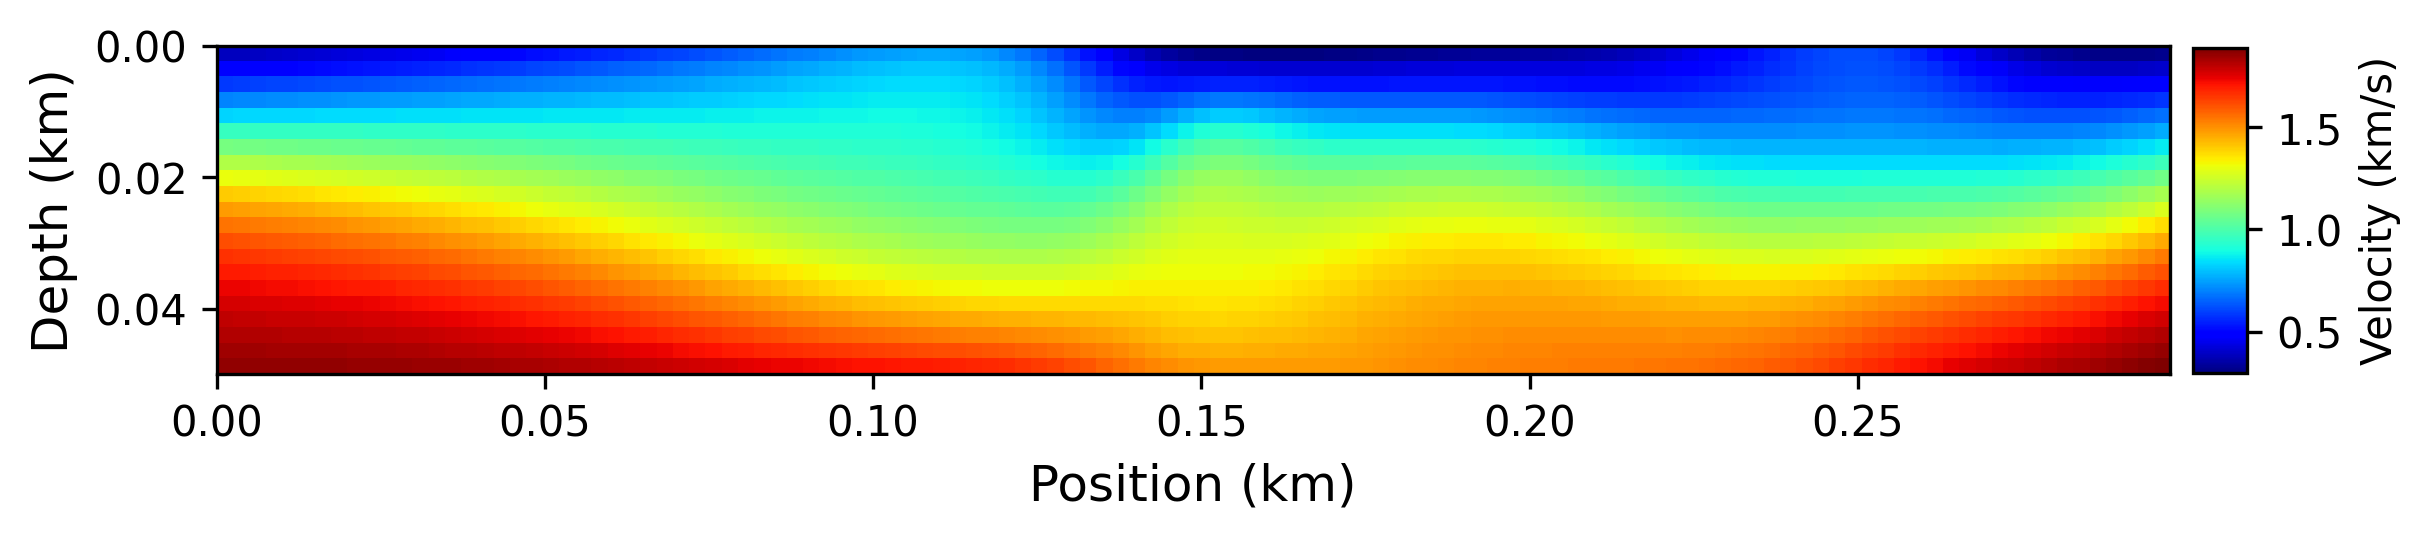
\includegraphics[width=0.9\textwidth]{figures/chap04_field_data/aqaba_pinn_tomo.png} 
 \caption{PINN predicted velocity model.}
 \label{fig:aqaba_pinn_tomo}
\end{figure}

 \begin{figure}
       \centering
       \begin{subfigure}[]{.9\textwidth}
               \centering
               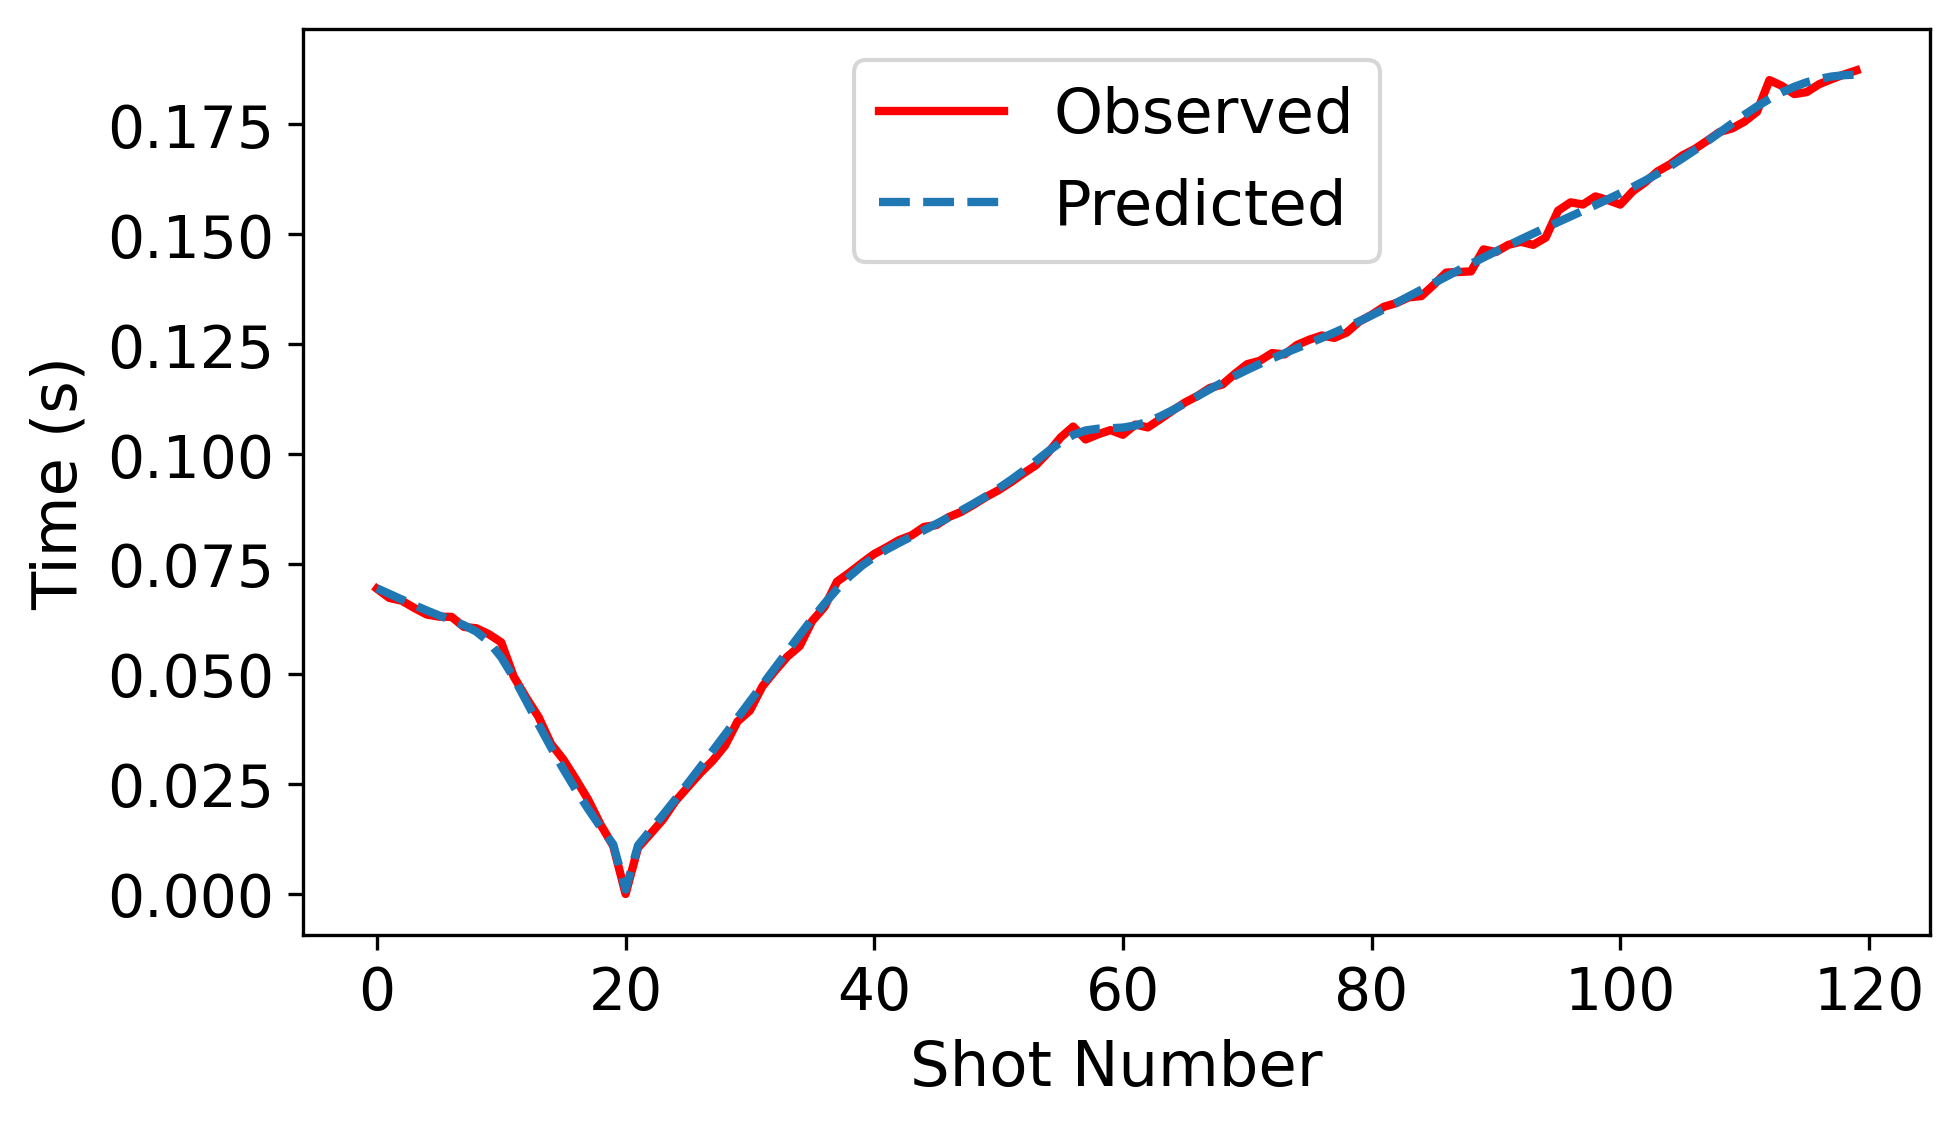
\includegraphics[width=0.9\textwidth]{figures/chap04_field_data/shot20.png} 
               \caption{}
               \label{fig:shot20}
       \end{subfigure}
       \begin{subfigure}[]{.9\textwidth}
               \centering
               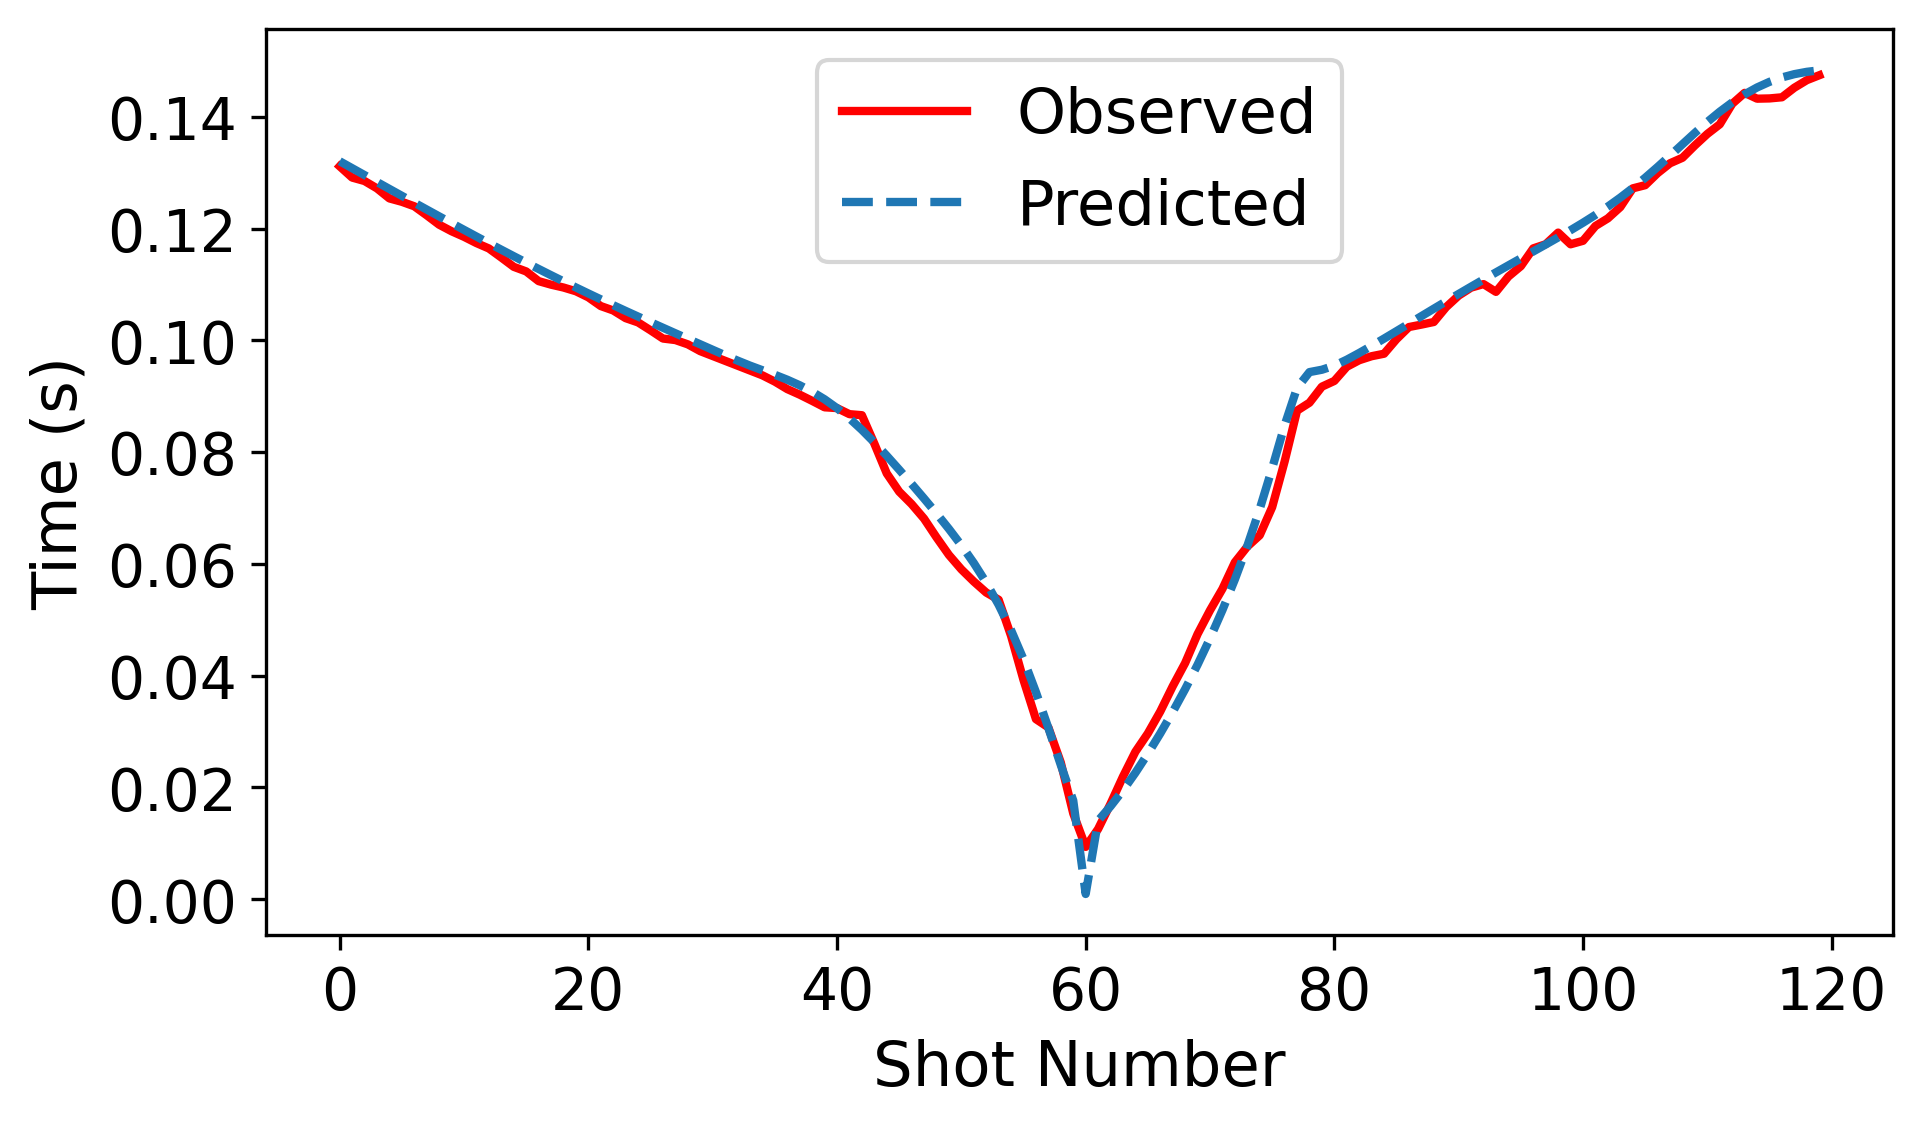
\includegraphics[width=0.9\textwidth]{figures/chap04_field_data/shot60.png}
               \caption{}
               \label{fig:shot60}
       \end{subfigure}
       \begin{subfigure}[]{.9\textwidth}
               \centering
               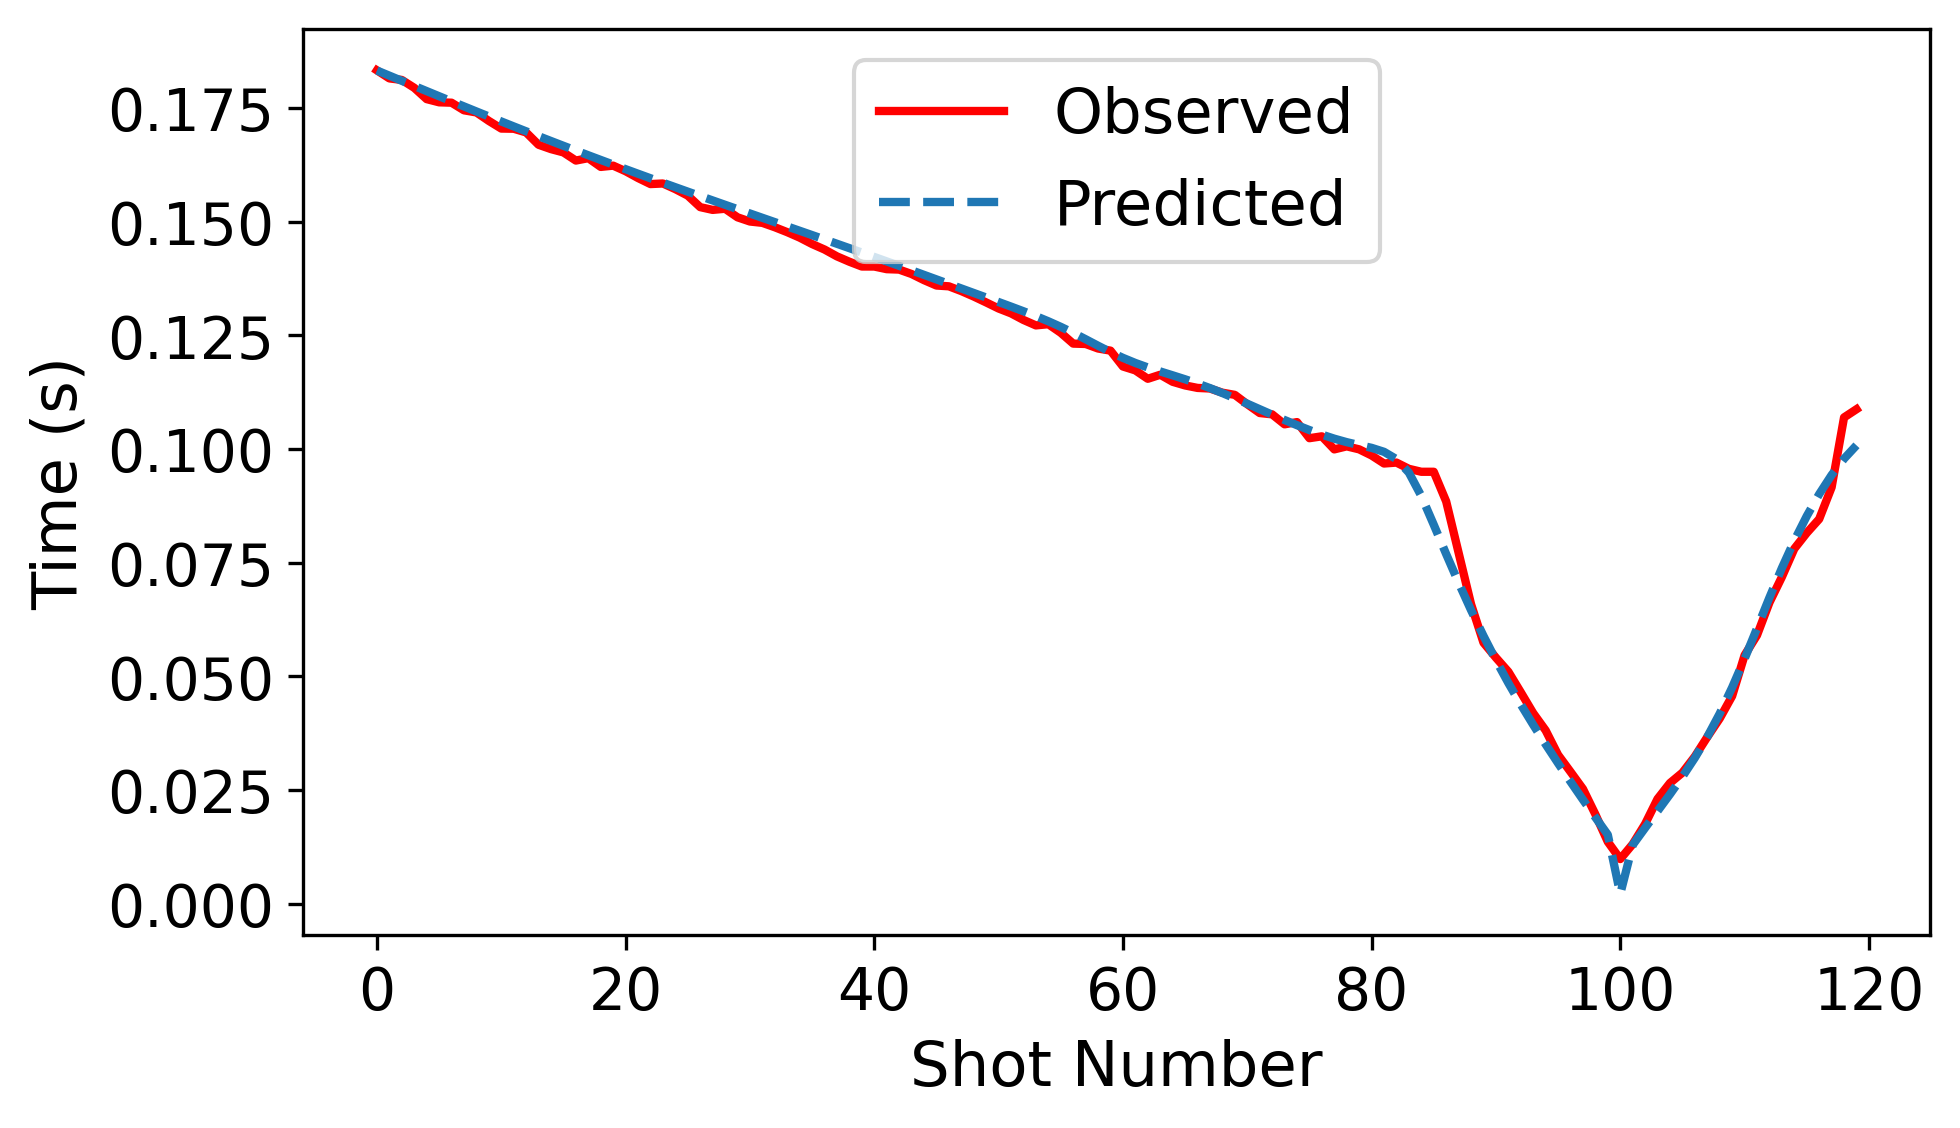
\includegraphics[width=0.9\textwidth]{figures/chap04_field_data/shot100.png}
               \caption{}
               \label{fig:shot100}
       \end{subfigure}
       \caption{A comparison between the observed traveltimes (solid red) and the PINN estimated ones (dashed blue) at the 20th (a), 60th (b), and the 100th (c) receivers.}
       \label{fig:shots}
\end{figure}